%%
%% This is file `tikzposter-template.tex',
%% generated with the docstrip utility.
%%
%% The original source files were:
%%
%% tikzposter.dtx  (with options: `tikzposter-template.tex')
%%
%% This is a generated file.
%%
%% Copyright (C) 2014 by Pascal Richter, Elena Botoeva, Richard Barnard, and Dirk Surmann
%%
%% This file may be distributed and/or modified under the
%% conditions of the LaTeX Project Public License, either
%% version 2.0 of this license or (at your option) any later
%% version. The latest version of this license is in:
%%
%% http://www.latex-project.org/lppl.txt
%%
%% and version 2.0 or later is part of all distributions of
%% LaTeX version 2013/12/01 or later.
%%


\documentclass{tikzposter} %Options for format can be included here

\usepackage{todonotes}

\usepackage[tikz]{bclogo}
\usepackage{lipsum}
\usepackage{amsmath}

\usepackage{booktabs}
\usepackage{longtable}
\usepackage[absolute]{textpos}
\usepackage[it]{subfigure}
\usepackage{graphicx}
\usepackage{cmbright}
%\usepackage[default]{cantarell}
%\usepackage{avant}
%\usepackage[math]{iwona}
\usepackage[math]{kurier}
\usepackage[T1]{fontenc}


%% add your packages here
\usepackage{hyperref}
% for random text
\usepackage{lipsum}
\usepackage[english]{babel}
\usepackage[pangram]{blindtext}

\colorlet{backgroundcolor}{blue!10}

 % Title, Author, Institute
\title{Bike Sharing Demand}
\author{Pratikshya Parajuli}
\institute{Ministry of Finance \\
	Government of Nepal
}
%\titlegraphic{logos/tulip-logo.eps}

%Choose Layout
\usetheme{Wave}

%\definebackgroundstyle{samplebackgroundstyle}{
%\draw[inner sep=0pt, line width=0pt, color=red, fill=backgroundcolor!30!black]
%(bottomleft) rectangle (topright);
%}
%
%\colorlet{backgroundcolor}{blue!10}

\begin{document}


\colorlet{blocktitlebgcolor}{blue!23}

 % Title block with title, author, logo, etc.
\maketitle

\begin{columns}
 % FIRST column
\column{0.5}% Width set relative to text width

%%%%%%%%%% -------------------------------------------------------------------- %%%%%%%%%%
 %\block{Main Objectives}{
%  	      	\begin{enumerate}
%  	      	\item Formalise research problem by extending \emph{outlying aspects mining}
%  	      	\item Proposed \emph{GOAM} algorithm is to solve research problem
%  	      	\item Utilise pruning strategies to reduce time complexity
%  	      	\end{enumerate}
%%  	      \end{minipage}
%}
%%%%%%%%%% -------------------------------------------------------------------- %%%%%%%%%%


%%%%%%%%%% -------------------------------------------------------------------- %%%%%%%%%%
\block{Introduction}{
    This is an automated system of renting bicycles. The process of obtaining membership, rental, and bike return is automated via a network of kiosk locations throughout a city.
    This project is required to combine historical usage patterns with \emph{weather} data inorder to forecast bike rental demandin Washington DC.
    
  	\begin{description}
  	\item[Target Goal]  Use information available before the rental period to predict hourly bike usage for the test set. 
  	\end{description}
}
%%%%%%%%%% -------------------------------------------------------------------- %%%%%%%%%%


%%%%%%%%%% -------------------------------------------------------------------- %%%%%%%%%%
\block{Data Summary}{
\begin{itemize}
   \item  Training Set provides the data and usage of the first 19 days of each month
    \item Test Set provides the data from the 20th to the end of the month
\end{itemize}

\begin{center}
    \begin{minipage}{0.5\linewidth}
    \centering
    \begin{tikzfigure}
      \centerline{\includegraphics[width=0.9\textwidth,height=0.5\textwidth]{graphics/img/Data_summary1.eps}}
    \end{tikzfigure}
    \end{minipage}
    \hfill
    \begin{minipage}{0.4\linewidth}
    \centering
    \begin{tikzfigure}
      \centerline{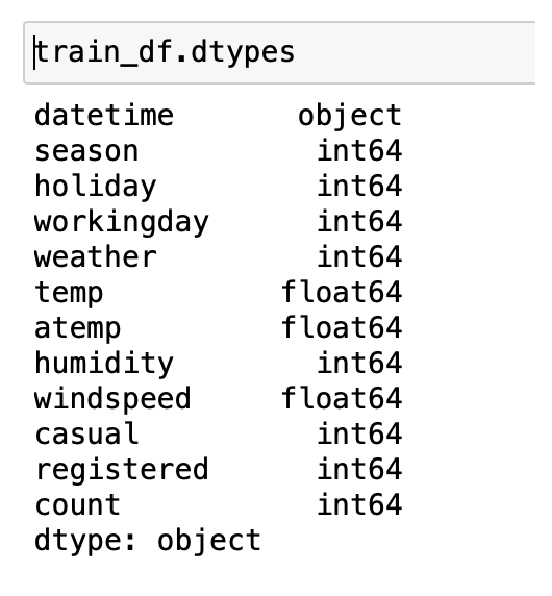
\includegraphics[width=0.9\textwidth,height=0.5\textwidth]{graphics/img/Data_summary2.eps}}
    \end{tikzfigure}%
    \end{minipage}
    \hfill
    
\end{center}
}
%%%%%%%%%% -------------------------------------------------------------------- %%%%%%%%%%


%%%%%%%%%% -------------------------------------------------------------------- %%%%%%%%%%

%\note{Note with default behavior}

%\note[targetoffsetx=12cm, targetoffsety=-1cm, angle=20, rotate=25]
%{Note \\ offset and rotated}

 % First column - second block


%%%%%%%%%% -------------------------------------------------------------------- %%%%%%%%%%
\block{Correlation Matrix}{
  	
  \begin{tikzfigure}
    \centerline{\includegraphics[width=0.4\textwidth,height=0.2\textwidth]{graphics/img/heatmap.eps}}
  \end{tikzfigure}
		
\begin{description}
  \item Based on the above heatmap, we can see that some of the features have no relation with the response variable. we can drop those columns.
  	\item\textcolor{orange} {humidity}, \textcolor{orange}{temp} are negatively correlated with count
  	\item
    There is a strong correlation between \textcolor{orange} {temp} and \textcolor{orange} {atemp}, if both are included in the model, it will cause multicollinearity problems, so one of the features must be deleted. We remove the atemp feature because it has a weaker correlation with count than temp.
    \item
    \textcolor{orange} {Casual}, \textcolor{orange}{Registered} are not considered and removed during model building 
    \item
    \textcolor{orange} {humidity}, \textcolor{orange}{temp} and \textcolor{orange} {windspeed} features are considered during future modelling
    \item 
    fill in the zero values in the windspeed feature: usage is high when the wind speed is 0, which may be caused by null filling. Therefore, a random forest model is used here to fill in the zero values.

\end{description}

}
%%%%%%%%%% -------------------------------------------------------------------- %%%%%%%%%%


% SECOND column
\column{0.5}
 %Second column with first block's top edge aligned with with previous column's top.

%%%%%%%%%% -------------------------------------------------------------------- %%%%%%%%%%
\block{Target Variable Analysis}{
\begin{description}
    \item
    As can be seen from the figure below, the target variable count has a right-skewed distribution. Since most machine learning techniques require the dependent variable to be normally distributed, variable transformation is required. One possible solution is to log-transform the count variable after removing outlier data points. The transformed data looks much better, approximately following a normal distribution.
\end{description}

\begin{tikzfigure}%[Overall architecture of \emph{GOAM} algorithm]
  \centerline{\includegraphics[width=0.4\textwidth,height=0.2\textwidth]{graphics/img/targetvariableanalysis.eps}}
\end{tikzfigure}
}
%%%%%%%%%% -------------------------------------------------------------------- %%%%%%%%%%
% Second column - first block


%%%%%%%%%% -------------------------------------------------------------------- %%%%%%%%%%
\block[titleleft]{Model Evaluation Results}
{
  \begin{description}
    \item Evaluation Indicators: root mean square error is required (Root Mean Squared Logarithmic Error, RMSLE) to evaluate the quality of the model. 
    \smallskip
    
    {$$ RMSLE = \sqrt{\frac{1}{n} \sum_{i=1}^n [\log(p_i + 1) - \log(a_i + 1)]^2} $$}
    Among them, $n$ is the number of samples in the test set, $p_i$ is the test value, and $a_i$ is the actual value. The smaller the root mean square error, the better the fitting effect of the data, and the closer the test value is to the actual value.
\end{description}
\vspace{.5cm}
\begin{description}
  	\item[Prediction with Linear Model] - Linear Regression, Ridge Regression, Lasso Regression, Logistic Regression, ElasticNet
\end{description}
\vspace{.5cm}

\begin{description}
    \item
    [Prediction with ensemble learning Model] - Bagging Regressor, Random Forest Regressor, Gradient Boosting Regressor, AdaBoost Regressor
\end{description}
\vspace{.5cm}
\centering
\begin{tabular}{ c | c | c | c }
  \toprule
    % after \\: \hline or \cline{col1-col2} \cline{col3-col4} ...
    Model     & Accuracy      \\
  \midrule
  Random Forest Regression        & 0.376319   \\
  Bagging Regression              & 0.395248    \\
  GBRT                            & 0.430378   \\
  AdaBoost Regression             & 0.703528   \\ 
  Ridge Regression                & 1.045335   \\
  Lasso Regression                & 1.045453 \\
  ElasticNet Regression           & 1.045489 \\
  Linear Regression               & 1.046341 \\
  Logistic Regression             & 1.131105 \\
  \bottomrule
  \end{tabular}

}
%%%%%%%%%% -------------------------------------------------------------------- %%%%%%%%%%


% Second column - second block
%%%%%%%%%% -------------------------------------------------------------------- %%%%%%%%%%
\block[titlewidthscale=1, bodywidthscale=1]
{Conclusion}
{
\begin{description}
  \item[Problem Definition]
  Use information available before the rental period to predict hourly bike usage for the test set.

  \item[Prediction Algorithm]
  Various linear model and ensemble learning algorithms are used for modelling.

  \item
  Results can be further enhanced
\end{description}
}
%%%%%%%%%% -------------------------------------------------------------------- %%%%%%%%%%


% Bottomblock
%%%%%%%%%% -------------------------------------------------------------------- %%%%%%%%%%
\colorlet{notebgcolor}{blue!20}
\colorlet{notefrcolor}{blue!20}
\note[targetoffsetx=8cm, targetoffsety=-4cm, angle=10, rotate=10,
radius=2cm, width=.16\textwidth]{
Acknowledgement
\begin{itemize}
    \item
    Tulip Lab
 \end{itemize}
}

%\note[targetoffsetx=8cm, targetoffsety=-10cm,rotate=0,angle=180,radius=8cm,width=.46\textwidth,innersep=.1cm]{
%Acknowledgement
%}

%\block[titlewidthscale=0.9, bodywidthscale=0.9]
%{Acknowledgement}{
%}
%%%%%%%%%% -------------------------------------------------------------------- %%%%%%%%%%

\end{columns}


%%%%%%%%%% -------------------------------------------------------------------- %%%%%%%%%%

\colorlet{notebgcolor}{blue!20}
\colorlet{notefrcolor}{blue!20}
\note[targetoffsetx=-13cm, targetoffsety=-12cm,rotate=0,angle=180,radius=8cm,width=.96\textwidth,innersep=.4cm]
{
\begin{minipage}{0.3\linewidth}
\centering
\includegraphics[width=24cm]{./graphics/logos/tulip-wordmark.eps}
\end{minipage}
\begin{minipage}{0.7\linewidth}
{ \centering
 The $11^{th}$ International Conference on Knowledge Science,
  Engineering and Management (KSEM 2018),
  17-19/08/2018, Changchun, China
}
\end{minipage}
}
%%%%%%%%%% -------------------------------------------------------------------- %%%%%%%%%%


\end{document}


